\documentclass[11pt,a4paper,center,notitlepage]{article}
\usepackage[backend=biber]{biblatex}

% Use Natbib reference style
%\usepackage{natbib}
 %\bibliographystyle{abbrvnat}

%\usepackage[backend=biber,style=authoryear,natbib=true]{biblatex} % Use the bibtex backend with the authoryear citation style (which resembles APA)

\addbibresource{mybib.bib} % The filename of the bibliography
% For tabular
\usepackage{tabularx}
%\usepackage{arydshln,leftidx,mathtools}
%
%\setlength{\dashlinedash}{.4pt}
%\setlength{\dashlinegap}{.8pt}

\usepackage[autostyle=true]{csquotes} % Required to generate language-dependent quotes in the bibliography

\usepackage{algorithm}
\usepackage{algpseudocode}
\usepackage[utf8]{inputenc} 
%\usepackage[T1]{fontenc}
\usepackage[english]{babel} 
\usepackage{color}
\usepackage{textcomp,multicol,enumerate,amsmath,amssymb,amsthm,eufrak,latexsym,makeidx}
\newcommand{\vertiii}[1]{{\left\vert\kern-0.25ex\left\vert\kern-0.25ex\left\vert #1 
    \right\vert\kern-0.25ex\right\vert\kern-0.25ex\right\vert}}
% For insert figure
\usepackage{subfig}
\usepackage{graphicx,epstopdf}

%% Color Reference
\usepackage[usenames,dvipsnames,svgnames,table]{xcolor}
\usepackage[colorlinks=true,
            linkcolor=blue,
            urlcolor=gray,
            citecolor=magenta]{hyperref}
            
\allowdisplaybreaks
% No page break in Bibliography
\numberwithin{equation}{section}
\addto{\captionsenglish}{%
  \renewcommand{\bibname}{References}
}


\textwidth=16 cm
\textheight=22 cm
\topmargin= -1 cm
\oddsidemargin=0 cm
\evensidemargin=1 cm
\parindent=0.6 cm
\parskip=1.5 mm
\newtheorem{lemma}{Lemma}[section]
\newtheorem{corollary}{Corollary}[section]
\newtheorem{definition}{Definition}[section]
\newtheorem{prop}{Proposition}[section]
\newtheorem{theorem}{Theorem}[section]
\newtheorem{prob}{Problem}[section]
\newtheorem{notation}{Notation}[section]
\newtheorem{remark}{Remark}[section]
\newtheorem{example}{Example}[section]
\newtheorem{ques}{Question}[section]
\newtheorem{sol}{Solution}[section]
\renewcommand{\thenotation}{}
\renewcommand{\thesection}{\arabic{section}}
\renewcommand{\thesubsection}
{\arabic{section}.\arabic{subsection}}
\pagestyle{plain}

% Reference
\newcommand{\er}{\eqref}

%\newtheorem{theorem}{Theorem}[section]
%\newtheorem{corollary}[theorem]{Corollary}
%\newtheorem{lemma}[theorem]{Lemma}
%\newtheorem{proposition}[theorem]{Proposition}

%\theoremstyle{definition}
%\newtheorem{definition}[theorem]{Definition}
%\newtheorem{remark}{Remark}
%\newtheorem{properties}{Properties}
%\newtheorem*{notation}{Notation}
%\newtheorem{counter}{Counter-example}
%\newtheorem{open}{Open problem}
%\newtheorem{conjecture}{Conjecture}


%% FONT commands
\newcommand{\txt}[1]{\;\text{ #1 }\;}%% Used in math only
\newcommand{\tbf}{\textbf}%% Bold face. Usage: \tbf{...}
\newcommand{\tit}{\textit}%% Italic
\newcommand{\tsc}{\textsc}%% Small caps
\newcommand{\trm}{\textrm}
\newcommand{\mbf}{\mathbf}%% Math bold
\newcommand{\mrm}{\mathrm}%% Math Roman
\newcommand{\bsym}{\boldsymbol}%% Bold math symbol
%%Macros for changing font size in math.
\newcommand{\scs}{\scriptstyle}%% as in subscript
\newcommand{\sss}{\scriptscriptstyle}%% as in sub-subscript
\newcommand{\txts}{\textstyle}
\newcommand{\dsps}{\displaystyle}
%%Macros for changing font size in text.
\newcommand{\fnz}{\footnotesize}
\newcommand{\scz}{\scriptsize}
%%\tiny<\scz<\fsz<\small<\large<\Large<\huge<\Huge
%%%%%%%%%%%%
%%%%%%%%%%%%
%% EQUATION commands
\newcommand{\be}{\begin{equation}}
\newcommand{\bel}[1]{\begin{equation}\label{#1}}
\newcommand{\ee}{\end{equation}}
%% This macro does not work with amstex.
\newcommand{\eqnl}[2]{\begin{equation}\label{#1}{#2}\end{equation}}
%%use not advisable; confusing
\newcommand{\barr}{\begin{eqnarray}}
\newcommand{\earr}{\end{eqnarray}}
\newcommand{\bars}{\begin{eqnarray*}}
\newcommand{\ears}{\end{eqnarray*}}
\newcommand{\nnu}{\nonumber \\}
%%%%%%%%%%%%%%%
%% Unnumbered THEOREM env.
%% New env. to be used for unnumbered theorem, lemma etc.
%%(but with specified name)

\newtheorem{subn}{\name}
\renewcommand{\thesubn}{}
\newcommand{\bsn}[1]{\def\name{#1}\begin{subn}}
\newcommand{\esn}{\end{subn}}
%%%%%%%%%%%%%%
%% NUMBERED THEOREM env.
%% Environments: theorem, lemma, corollary defintion and
%%related commands,
%% designed to provide consecutive numbering of these forms.


\newtheorem{sub}{\name}[section]
\newcommand{\dn}[1]{\def\name{#1}}

%%used in conjuction with sub or subn.

\newcommand{\bs}{\begin{sub}}
\newcommand{\es}{\end{sub}}
\newcommand{\bsl}[1]{\begin{sub}\label{#1}}
	
%% the above must be preceeded by \dn (name definition),
%% however this is superceded by the list of commands bth etc. below.
%%%%%%%%%%%%
%% NUMBERED THEOREM env. (cont.)
%% List of commands derived from 'sub' env. for theorem, lemma etc.
%% designed to provide consecutive numbering of these forms.
\newcommand{\bth}[1]{\def\name{Theorem}\begin{sub}\label{t:#1}}
\newcommand{\blemma}[1]{\def\name{Lemma}\begin{sub}\label{l:#1}}
\newcommand{\bcor}[1]{\def\name{Corollary}\begin{sub}\label{c:#1}}	
\newcommand{\bdef}[1]{\def\name{Definition}\begin{sub}\label{d:#1}}
\newcommand{\bprop}[1]{\def\name{Proposition}\begin{sub}\label{p:#1}}	
%% ARRAY commands.%%%%%%%%%%%%%%%%%%%%%%%%%%%%%%%%%%
%% RERERENCE commands.
%% \newcommand{\R}[1]{(\ref{#1})}

\newcommand{\R}{\eqref}
\newcommand{\re}{\eqref}
\newcommand{\rth}[1]{Theorem~\ref{t:#1}}
\newcommand{\rlemma}[1]{Lemma~\ref{l:#1}}
\newcommand{\rcor}[1]{Corollary~\ref{c:#1}}
\newcommand{\rdef}[1]{Definition~\ref{d:#1}}
\newcommand{\rprop}[1]{Proposition~\ref{p:#1}}
%%%%%%%%%%%
\newcommand{\BA}{\begin{array}}
\newcommand{\EA}{\end{array}}
\newcommand{\BAN}{\renewcommand{\arraystretch}{1.2}
\setlength{\arraycolsep}{2pt}\begin{array}}
\newcommand{\BAV}[2]{\renewcommand{\arraystretch}{#1}
\setlength{\arraycolsep}{#2}\begin{array}}
%Note: The first variable gives the amount of stretching:
%(#1) x default.
%For instance #1=1.2 means a 20% stretching.
%The second variable should be
%written for instance in the form  4pt ; here the default is 5pt
%\newcommand{\EAN}{\end{array}\setlength{\arraycolsep}{5pt}}
\newcommand{\BSA}{\begin{subarray}}
\newcommand{\ESA}{\end{subarray}}	
%Note: These are used in subscripts as well as superscripts.
%They work essentially like 'array'.

\newcommand{\BAL}{\begin{aligned}}
	\newcommand{\EAL}{\end{aligned}}
\newcommand{\BALG}{\begin{alignat}}
	\newcommand{\EALG}{\end{alignat}}
%% the abbrev. does not work with latex2e
\newcommand{\BALGN}{\begin{alignat*}}
	\newcommand{\EALGN}{\end{alignat*}}
%% the abbrev. does not work with latex2e
%% The 'aligned' environment must be placed inside an 'equation' env.
%% in the same way as the array.
%% One could use also the 'align' env. or the 'alignat' env.
%% However in this case each line is numbered, unless '\notag' is used.
%% The 'alignat'
%% has a slightly different format (the number of columns must be %%specified in advance)
%% but it has the advantage that the distance between columns
%%is at our disposition.
%% (The default would be zero distance.) Using 'alignat*' we can have %%the advantages
%% of alignat plus the situation where separate lines are not numbered.
%% However in this case there is no numbering at all
%%(unless we provide a tag).
%%%%%%%%%%
%% PROOF, REMARK etc.
\newcommand{\note}[1]{\noindent\textit{#1.}\hspace{2mm}}
\newcommand{\Proof}{\note{Proof}}
%\newcommand{\qed}{\hspace{10mm}\hfill $\square$}
%\newcommand{\qed}{\\${}$ \hfill $\square$}
\newcommand{\Remark}{\note{Remark}}
%%%%%%%% Style command.
\newcommand{\modin}{$\,$\\[-4mm] \indent}
%% To be used after \section in order to start new line with \indent.
%%%%%%%%%%%%
%% MATHEMATICAL symbols
\newcommand{\forevery}{\quad \forall}
\newcommand{\set}[1]{\{#1\}}
\newcommand{\setdef}[2]{\{\,#1:\,#2\,\}}
\newcommand{\setm}[2]{\{\,#1\mid #2\,\}}
%% Arrows
\newcommand{\mt}{\mapsto}
\newcommand{\lra}{\longrightarrow}
\newcommand{\lla}{\longleftarrow}
\newcommand{\llra}{\longleftrightarrow}
\newcommand{\Lra}{\Longrightarrow}
\newcommand{\Lla}{\Longleftarrow}
\newcommand{\Llra}{\Longleftrightarrow}
\newcommand{\warrow}{\rightharpoonup}

%% Brackets, delimiters
\newcommand{\paran}[1]{\left (#1 \right )}
%% adjustable parantheses
\newcommand{\sqbr}[1]{\left [#1 \right ]}
%% adjustable square brackets
\newcommand{\curlybr}[1]{\left \{#1 \right \}}
%% adjustable curly brackets
\newcommand{\abs}[1]{\left |#1\right |}

%% adjustable vertical delimiters
\newcommand{\norm}[1]{\left \|#1\right \|}

%% adjustable norm
\newcommand{\paranb}[1]{\big (#1 \big )}

%% non-adjustable parantheses (big)
\newcommand{\lsqbrb}[1]{\big [#1 \big ]}

%% non-adjustable square brackets (big)
\newcommand{\lcurlybrb}[1]{\big \{#1 \big \}}

%% non-adjustable curly brackets(big)
\newcommand{\absb}[1]{\big |#1\big |}

%% non-adjustable vertical delimiters(big)
\newcommand{\normb}[1]{\big \|#1\big \|}

%% non-adjustable norm (big)
\newcommand{	\paranB}[1]{\Big (#1 \Big )}

%% non-adjustable parantheses (Big)
\newcommand{\absB}[1]{\Big |#1\Big |}

%% non-adjustable vertical delimiters(Big)
\newcommand{\normB}[1]{\Big \|#1\Big \|}%% non-adjustable norm (Big)
\newcommand{\produal}[1]{\langle #1 \rangle}%% the pairing of X' and X
%%%%%%%%%%%%%%%%%
%% Adjustable parantheses etc. in a different DEFINITION format.
%\def\adp(#1){\left (#1 \right )}%% adjustable parantheses
%\def\adsb(#1){\left [#1\right ]}%% adjustable square brackets
%\def\adcb(#1){\left \{#1\right \}}%% adjustable curly brackets
%\def\abs|#1|{\left |#1\right |}%% adjustable vertical delimiters
%%%%%%%%%%%%%%%%
%% More mathematical symbols
\newcommand{\thkl}{\rule[-.5mm]{.3mm}{3mm}}
\newcommand{\thknorm}[1]{\thkl #1 \thkl\,}
\newcommand{\trinorm}[1]{|\!|\!| #1 |\!|\!|\,}
\newcommand{\bang}[1]{\langle #1 \rangle}%% angle bracket
\def\angb<#1>{\langle #1 \rangle}%% angle bracket
%% The two last lines yield the same result.
%% The second is used as follows: \angb<a,b>
\newcommand{\vstrut}[1]{\rule{0mm}{#1}}
\newcommand{\rec}[1]{\frac{1}{#1}}
%% OPERATOR names.
%% OPERATOR names.
\newcommand{\opname}[1]{\mbox{\rm #1}\,}
\newcommand{\supp}{\opname{supp}}
\newcommand{\dist}{\opname{dist}}
\newcommand{\myfrac}[2]{{\displaystyle \frac{#1}{#2} }}
\newcommand{\myint}[2]{{\displaystyle \int_{#1}^{#2}}}
\newcommand{\mysum}[2]{{\displaystyle \sum_{#1}^{#2}}}
\newcommand {\dint}{{\displaystyle \myint\!\!\myint}}%%%%%%%%%%
%%%%%%% SPACE commands
\newcommand{\q}{\quad}
\newcommand{\qq}{\qquad}
\newcommand{\hsp}[1]{\hspace{#1mm}}
\newcommand{\vsp}[1]{\vspace{#1mm}}
%%%%%%%%%%%
%% ABREVIATIONS
\newcommand{\ity}{\infty}
\newcommand{\prt}{\partial}
\newcommand{\sms}{\setminus}
\newcommand{\ems}{\emptyset}
\newcommand{\ti}{\times}
\newcommand{\pr}{^\prime}
\newcommand{\ppr}{^{\prime\prime}}
\newcommand{\tl}{\tilde}
\newcommand{\sbs}{\subset}
\newcommand{\sbeq}{\subseteq}
\newcommand{\nind}{\noindent}
\newcommand{\ind}{\indent}
\newcommand{\ovl}{\overline}
\newcommand{\unl}{\underline}
\newcommand{\nin}{\not\in}
\newcommand{\pfrac}[2]{\genfrac{(}{)}{}{}{#1}{#2}}

%% frac with parantheses.
%%%%%%%%%%%
%%%%%%%%%%%%%

%%Macros for Greek letters.
\def\ga{\alpha}     \def\gb{\beta}       \def\gg{\gamma}
\def\gc{\chi}       \def\gd{\delta}      \def\gep{\epsilon}
\def\gth{\theta}                         \def\vge{\varepsilon}
\def\gf{\varphi}       \def\vgf{\varphi}    \def\gh{\eta}
\def\gi{\iota}      \def\gk{\kappa}      \def\gl{\lambda}
\def\gm{\mu}        \def\gn{\nu}         \def\gp{\pi}
\def\vgp{\varpi}    \def\gr{\gd}        \def\vgr{\varrho}
\def\gs{\sigma}     \def\vgs{\varsigma}  \def\gt{\tau}
\def\gu{\upsilon}   \def\gv{\vartheta}   \def\gw{\omega}
\def\gx{\xi}        \def\gy{\psi}        \def\gz{\zeta}
\def\Gg{\Gamma}     \def\Gd{\Delta}      \def\Gf{\Phi}
\def\Gth{\Theta}
\def\Gl{\Lambda}    \def\Gs{\Sigma}      \def\Gp{\Pi}
\def\Gw{\Omega}     \def\Gx{\Xi}         \def\Gy{\Psi}

%%Macros for calligraphic letters.
\def\CS{{\mathcal S}}   \def\CM{{\mathcal M}}   \def\CN{{\mathcal N}}
\def\CR{{\mathcal R}}   \def\CO{{\mathcal O}}   \def\CP{{\mathcal P}}
\def\CA{{\mathcal A}}   \def\CB{{\mathcal B}}   \def\CC{{\mathcal C}}
\def\CD{{\mathcal D}}   \def\CE{{\mathcal E}}   \def\CF{{\mathcal F}}
\def\CG{{\mathcal G}}   \def\CH{{\mathcal H}}   \def\CI{{\mathcal I}}
\def\CJ{{\mathcal J}}   \def\CK{{\mathcal K}}   \def\CL{{\mathcal L}}
\def\CT{{\mathcal T}}   \def\CU{{\mathcal U}}   \def\CV{{\mathcal V}}
\def\CZ{{\mathcal Z}}   \def\CX{{\mathcal X}}   \def\CY{{\mathcal Y}}
\def\CW{{\mathcal W}} \def\CQ{{\mathcal Q}}
%%%%%
%%Macros for 'blackboard' letters (See (27) for display.)
\def\BBA {\mathbb A}   \def\BBb {\mathbb B}    \def\BBC {\mathbb C}
\def\BBD {\mathbb D}   \def\BBE {\mathbb E}    \def\BBF {\mathbb F}
\def\BBG {\mathbb G}   \def\BBH {\mathbb H}    \def\BBI {\mathbb I}
\def\BBJ {\mathbb J}   \def\BBK {\mathbb K}    \def\BBL {\mathbb L}
\def\BBM {\mathbb M}   \def\BBN {\mathbb N}    \def\BBO {\mathbb O}
\def\BBP {\mathbb P}   \def\BBR {\mathbb R}    \def\BBS {\mathbb S}
\def\BBT {\mathbb T}   \def\BBU {\mathbb U}    \def\BBV {\mathbb V}
\def\BBW {\mathbb W}   \def\BBX {\mathbb X}    \def\BBY {\mathbb Y}
\def\BBZ {\mathbb Z}

%%Macros for Ghotic (Fraktur) letters.
\def\GTA {\mathfrak A}   \def\GTB {\mathfrak B}    \def\GTC {\mathfrak C}
\def\GTD {\mathfrak D}   \def\GTE {\mathfrak E}    \def\GTF {\mathfrak F}
\def\GTG {\mathfrak G}   \def\GTH {\mathfrak H}    \def\GTI {\mathfrak I}
\def\GTJ {\mathfrak J}   \def\GTK {\mathfrak K}    \def\GTL {\mathfrak L}
\def\GTM {\mathfrak M}   \def\GTN {\mathfrak N}    \def\GTO {\mathfrak O}
\def\GTP {\mathfrak P}   \def\GTR {\mathfrak R}    \def\GTS {\mathfrak S}
\def\GTT {\mathfrak T}   \def\GTU {\mathfrak U}    \def\GTV {\mathfrak V}
\def\GTW {\mathfrak W}   \def\GTX {\mathfrak X}    \def\GTY {\mathfrak Y}
\def\GTZ {\mathfrak Z}   \def\GTQ {\mathfrak Q}
\def\sign{\mathrm{sign\,}}
\def\bdw{\prt\Gw\xspace}
\def\nabu{|\nabla u|}
\def\tr{\mathrm{tr\,}}
\def\gap{{\ga_+}}
\def\gan{{\ga_-}}

\def\N{\mathbb{N}}
\def\Z{\mathbb{Z}}
\def\Q{\mathbb{Q}}
\def\R{\mathbb{R}}


\def\Proof.{{\bf{Proof. }}}
\def\End{\hspace{1cm} $\Box$\\}


\renewcommand{\baselinestretch}{1.1}

\let\e=\varepsilon
\let\vp=\varphi
\let\t=\tilde
\let\ol=\overline
\let\ul=\underline
\let\.=\cdot
\let\0=\emptyset
\let\mc=\mathcal
\def\ex{\exists\;}
\def\fa{\forall\;}
\def\se{\ \Leftarrow\ }
\def\solose{\ \Rightarrow\ }
\def\sse{\ \Leftrightarrow\ }
\def\meno{\,\backslash\,}
\def\pp{,\dots,}
\def\D{\mc{D}}
\def\O{\Omega}


\def\loc{\text{\rm loc}}
\def\diam{\text{\rm diam}}
\def\dist{\text{\rm dist}}
\def\dv{\text{\rm div}}
\def\sign{\text{\rm sign}}
\def\supp{\text{\rm supp}}
\def\tr{\text{\rm Tr}}
\def\vec{\text{\rm vec}}
\def\inter{\text{\rm int\,}}
\def\norma#1{\|#1\|_\infty}

\newcommand{\esssup}{\mathop{\rm ess{\,}sup}}
\newcommand{\essinf}{\mathop{\rm ess{\,}inf}}
\newcommand{\su}[2]{\genfrac{}{}{0pt}{}{#1}{#2}}

\def\eq#1{{\rm(\ref{eq:#1})}}
\def\thm#1{Theorem \ref{thm:#1}}
\def\seq#1{(#1_n)_{n\in\N}}
\def\limn{\lim_{n\to\infty}}


\def\PP{\mc{P}}
\def\pe{principal eigenvalue}
\def\MP{maximum principle}
\def\SMP{strong maximum principle}
\def\l{\lambda_1}

\def\bq{\begin{equation}}
\def\eq{\end{equation}}

\def\l{\label}

\newenvironment{formula}[1]{\begin{equation}\label{eq:#1}}	{\end{equation}\noindent}

\title{Notes $\star$ Analyse Num\'erique - Part II: Implementation of the Finite Elements $\star$ Examination - Numerical Validation}
\author{Nguyen Quan Ba Hong\footnote{Master 2 Student at UFR math\'ematiques, Universit\'e de Rennes 1, Beaulieu - B\^atiment 22 et 23, 263 avenue du G\'en\'eral Leclerc, 35042 Rennes CEDEX, France.\newline
E-mail: \texttt{nguyenquanbahong@gmail.com} \newline
Blog: \texttt{\url{www.nguyenquanbahong.com}} \newline 
Copyright \copyright\ 2016-2018 by Nguyen Quan Ba Hong. This document may be copied freely for the purposes of education and non-commercial research. Visit my site to get more.}}
\begin{document}
\maketitle
\begin{abstract}
This context includes the materials given in the course \textit{Finite Element Method} in the Master 2 Fundamental Mathematics program 2018-2019, with my \textsc{Matlab} scripts provided.
\end{abstract}
%\textbf{Mathematics Subject Classification (2010):} 
%
%\noindent
%\textbf{Keywords:} \emph{}
\maketitle
\textbf{Brief introduction.} ``This lecture is a numerical counterpart to \textit{Sobolev spaces \& elliptic equations}. In the first part, after some reminders on linear elliptic partial differential equations, the approximation of the associated solutions by the finite element methods is investigated. Their construction and their analysis are described in one and two dimensions. The second part of the lectures consists in defining a generic strategy for the implementation of the method based on the variational formulation. A program is written in \textsc{Matlab} (implementable with \textsc{Matlab} or \textsc{Octave}).''
\newpage
\tableofcontents
\newpage

\section*{Introduction}
To validate a code, several strategies are used:
\begin{enumerate}
\item Check each function or elementary part of the code by application to very simple examples where the results can be verified by hand calculation.
\item Check the obtained results in configurations where the exact solution is known.
\item Check the asymptotic behavior. For example, you can check the asymptotic behavior of the finite-element error with respect to the discretization parameter $h$. In the case of a PDE the solution of which is known, you will plot the error with respect to the discretization parameter $h$ in ``loglog'' scale.
\end{enumerate}
The following exercises which involve these strategies are proposed.

\section{Validation of the Assembling Procedure}
In order to validate your programming in the context of iso-parametric $\mathbb{P}_1$ finite elements, you will write a script which calculates the mass and stiffness matrices for the following mesh:
\begin{verbatim}
coords_ = [0,0;.5,0;1,0;0,.5;.5,.5;1,.5;0,1;.5,1;1,1];
triangles_ = [1,2,4;2,5,4;2,3,5;3,6,5;4,5,7;5,8,7;5,6,8;6,9,8];
\end{verbatim}
To be sure of the correctness of the numerical results, you can calculate some components of the matrices by hand. The results and your analysis of them will be written in the script as ending comments. Finally, you will also justify the choice of the quadrature rule for each matrix. This justification will be expressed in the script, as a comment where it appears to be the most relevant for you.

N.B.: We remember the definition of the mass matrix 
\begin{align}
{M_{ij}} = \int_{{\Omega _h}} {{\varphi _i}\left( x \right){\varphi _j}\left( x \right)dx} ,\hspace{2mm} \forall \left( {i,j} \right),
\end{align}
and the stiffness matrix
\begin{align}
{R_{ij}} = \int_{{\Omega _h}} {\nabla {\varphi _i}\left( x \right) \cdot \nabla {\varphi _j}\left( x \right)dx} ,\hspace{2mm} \forall \left( {i,j} \right),
\end{align}
where $\left(i,j\right)$ designates the couples of nodes of the mesh, $\Omega _h$ the domain as described by the triangles of the mesh and ${\left\{ {{\varphi _i}} \right\}_i}$ the basis functions of the finite-element interpolation.

Running the following codes in the main script
\begin{verbatim}
%% Compute the Mass Matrix 
% Use the P_1 nodal quadrature formula
M =  assemble_matrix('Id', 'Id', 'f_one', mesh_geo, 1, 1)
% Use the P_3 nodal quadrature formula
M =  assemble_matrix('Id', 'Id', 'f_one', mesh_geo, 1, 2)

%% Compute the Stiffness Matrix
R1 = assemble_matrix('D1', 'D1', 'f_one', mesh_geo, 1, 1);
R2 = assemble_matrix('D2', 'D2', 'f_one', mesh_geo, 1, 1);
R = R1 + R2
\end{verbatim}
gives us the following mass and stiffness matrices:
\begin{verbatim}
M =

  Columns 1 through 3

   0.041666666666667                   0                   0
                   0   0.125000000000000                   0
                   0                   0   0.083333333333333
                   0                   0                   0
                   0                   0                   0
                   0                   0                   0
                   0                   0                   0
                   0                   0                   0
                   0                   0                   0

  Columns 4 through 6

                   0                   0                   0
                   0                   0                   0
                   0                   0                   0
   0.125000000000000                   0                   0
                   0   0.250000000000000                   0
                   0                   0   0.125000000000000
                   0                   0                   0
                   0                   0                   0
                   0                   0                   0

  Columns 7 through 9

                   0                   0                   0
                   0                   0                   0
                   0                   0                   0
                   0                   0                   0
                   0                   0                   0
                   0                   0                   0
   0.083333333333333                   0                   0
                   0   0.125000000000000                   0
                   0                   0   0.041666666666667


M =

  Columns 1 through 3

   0.020833333333333   0.010416666666667                   0
   0.010416666666667   0.062500000000000   0.010416666666667
                   0   0.010416666666667   0.041666666666667
   0.010416666666667   0.020833333333333                   0
                   0   0.020833333333333   0.020833333333333
                   0                   0   0.010416666666667
                   0                   0                   0
                   0                   0                   0
                   0                   0                   0

  Columns 4 through 6

   0.010416666666667                   0                   0
   0.020833333333333   0.020833333333333                   0
                   0   0.020833333333333   0.010416666666667
   0.062500000000000   0.020833333333333                   0
   0.020833333333333   0.125000000000000   0.020833333333333
                   0   0.020833333333333   0.062500000000000
   0.010416666666667   0.020833333333333                   0
                   0   0.020833333333333   0.020833333333333
                   0                   0   0.010416666666667

  Columns 7 through 9

                   0                   0                   0
                   0                   0                   0
                   0                   0                   0
   0.010416666666667                   0                   0
   0.020833333333333   0.020833333333333                   0
                   0   0.020833333333333   0.010416666666667
   0.041666666666667   0.010416666666667                   0
   0.010416666666667   0.062500000000000   0.010416666666667
                   0   0.010416666666667   0.020833333333333


R =

  Columns 1 through 3

   1.000000000000000  -0.500000000000000                   0
  -0.500000000000000   2.000000000000000  -0.500000000000000
                   0  -0.500000000000000   1.000000000000000
  -0.500000000000000                   0                   0
                   0  -1.000000000000000                   0
                   0                   0  -0.500000000000000
                   0                   0                   0
                   0                   0                   0
                   0                   0                   0

  Columns 4 through 6

  -0.500000000000000                   0                   0
                   0  -1.000000000000000                   0
                   0                   0  -0.500000000000000
   2.000000000000000  -1.000000000000000                   0
  -1.000000000000000   4.000000000000000  -1.000000000000000
                   0  -1.000000000000000   2.000000000000000
  -0.500000000000000                   0                   0
                   0  -1.000000000000000                   0
                   0                   0  -0.500000000000000

  Columns 7 through 9

                   0                   0                   0
                   0                   0                   0
                   0                   0                   0
  -0.500000000000000                   0                   0
                   0  -1.000000000000000                   0
                   0                   0  -0.500000000000000
   1.000000000000000  -0.500000000000000                   0
  -0.500000000000000   2.000000000000000  -0.500000000000000
                   0  -0.500000000000000   1.000000000000000
\end{verbatim}
which are exactly the results given in the script \verb|test_assemble_matrix_etu_0.m| in \cite{1}. \hfill $\square$

\begin{remark}
To compute the mass matrix $M$, the $\mathbb{P}_3$ nodal quadrature formula must be used rather than the $\mathbb{P}_1$ nodal quadrature formula, since the polynomials in the involving integrand has the degree two.
\end{remark}
Moreover, the Gaussian quadrature formulas can be used instead of the nodal quadrature formulas to increase the accuracy of the assembling procedure for the finite-element right hand side vector.

\section{Validation of the Convergence Order of the Finite-Element Method}
We consider the problem
\begin{equation}
\left\{ \begin{split}
 - \Delta u + u &= f, & \mbox{ on } \Omega ,\\
\frac{{\partial u}}{{\partial n}} &= 0, & \mbox{ on } \partial \Omega ,
\end{split} \right.
\end{equation}
where $\Omega$ is the square $\left[0,1\right]\times \left[0,1\right]$, and the function $f$ is chosen such that the exact solution is 
\begin{align}
u\left( x \right) = \cos \left( {\pi {x_1}} \right)\cos \left( {\pi {x_2}} \right).
\end{align}

\begin{prob}\label{prob2.1}
Write a function which solves the problem by application of the finite-element method (iso-parametric $\mathbb{P}_1$ or $\mathbb{P}_2$) with the following entries: the discretization parameter $h$ of the mesh and the degree of the interpolation. This function builds or loads the mesh ($\mathbb{P}_1$ or $\mathbb{P}_2$) according to the discretization parameter $h$, then assemblies the matrix of the variational approximation, and finally solves the linear system. The output of the function is a vector which contains the approximation of $u$ at the nodes of the mesh, and the coordinates of these nodes.
\end{prob}

\begin{proof}[Solution]
See Sec. \ref{sec3.4}. Running the following command lines in the main script
\begin{verbatim}
[X, nodes] = solve_Neumann_BVP(mesh_geo, 100, degree_FE);
figure
trisurf(mesh_geo.triangles, mesh_geo.coords(:,1), mesh_geo.coords(:,2), X);
\end{verbatim}
with \verb|degree_FE=1,2| and some refinements, gives us 
\newpage
\begin{figure}[H]
\centering
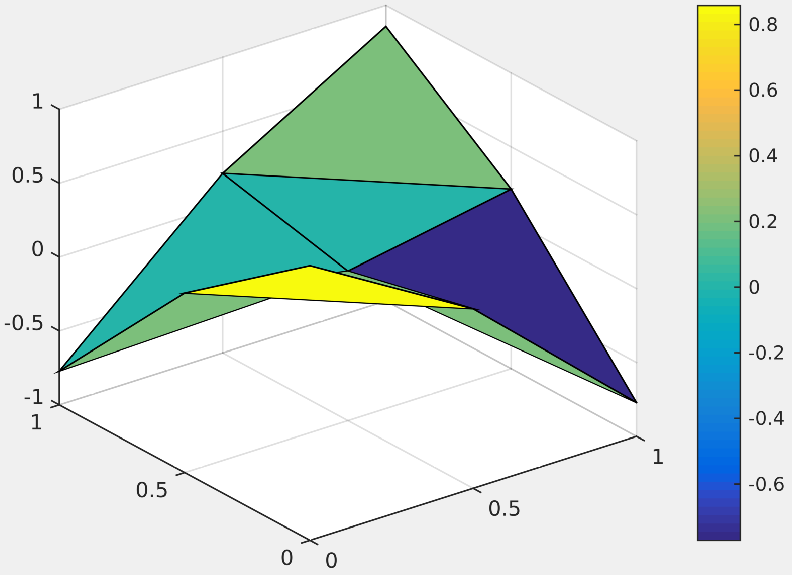
\includegraphics[scale=0.9]{appro_solution_1_P1}
\caption{$\mathbb{P}_1$ approximate solution.}
\end{figure} 

\begin{figure}[H]
\centering
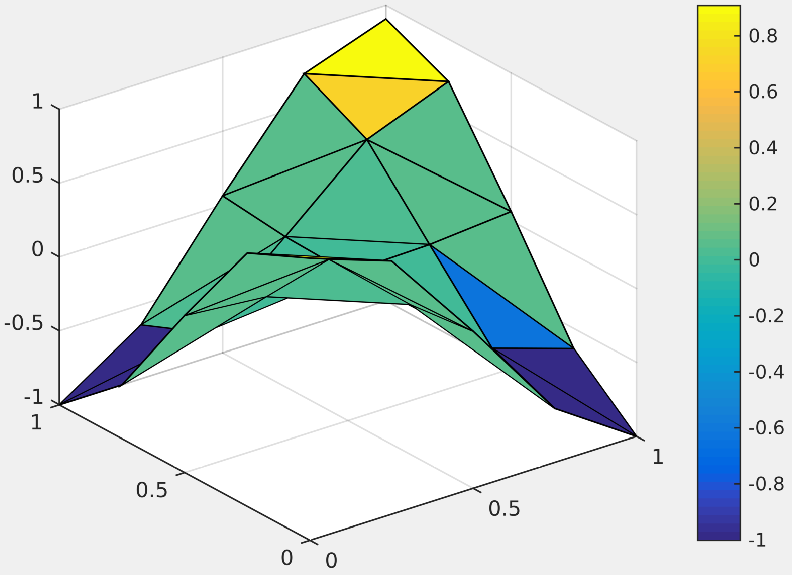
\includegraphics[scale=0.9]{appro_solution_2_P1}
\caption{$\mathbb{P}_1$ approximate solution.}
\end{figure} 

\begin{figure}[H]
\centering
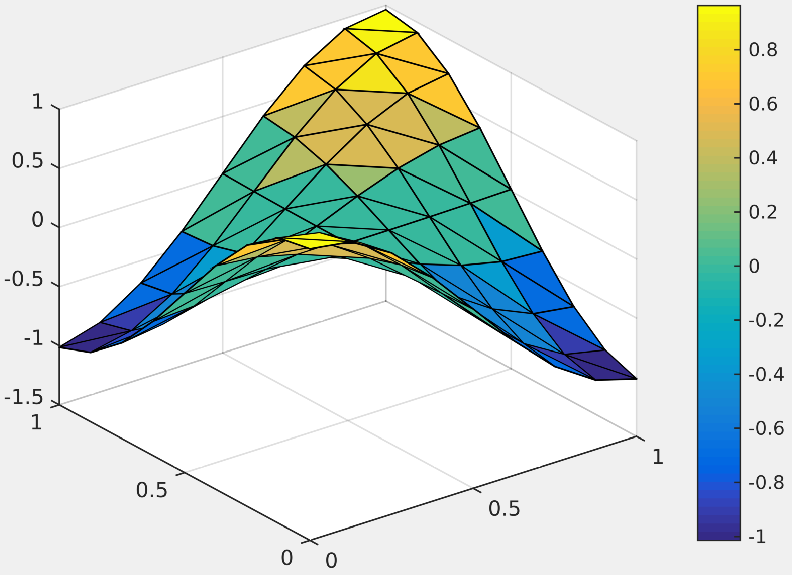
\includegraphics[scale=0.9]{appro_solution_3_P1}
\caption{$\mathbb{P}_1$ approximate solution.}
\end{figure} 

\begin{figure}[H]
\centering
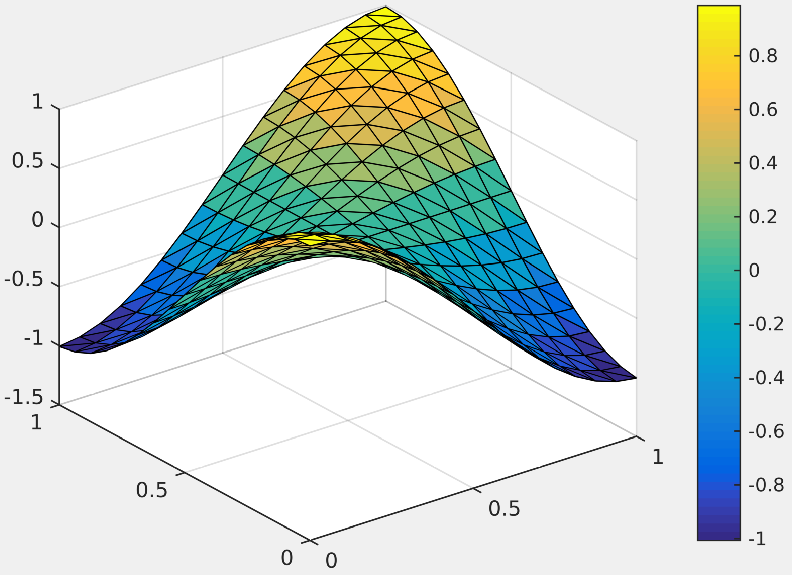
\includegraphics[scale=0.9]{appro_solution_4_P1}
\caption{$\mathbb{P}_1$ approximate solution.}
\end{figure} 

\begin{figure}[H]
\centering
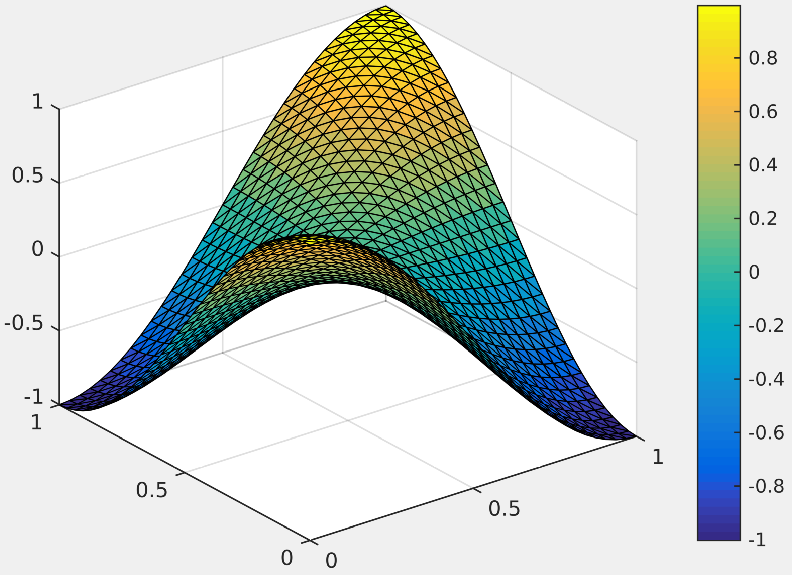
\includegraphics[scale=0.9]{appro_solution_5_P1}
\caption{$\mathbb{P}_1$ approximate solution.}
\end{figure} 

\begin{figure}[H]
\centering
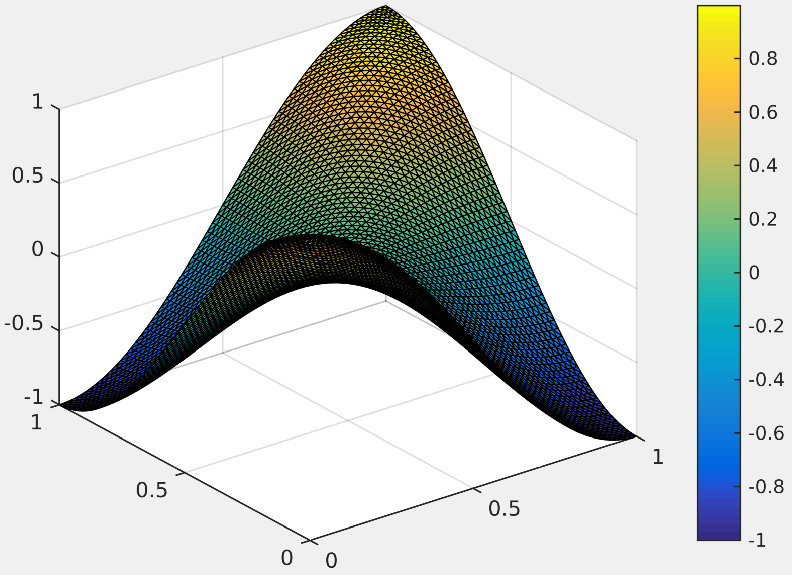
\includegraphics[scale=0.9]{appro_solution_6_P1}
\caption{$\mathbb{P}_1$ approximate solution.}
\end{figure} 

\begin{figure}[H]
\centering
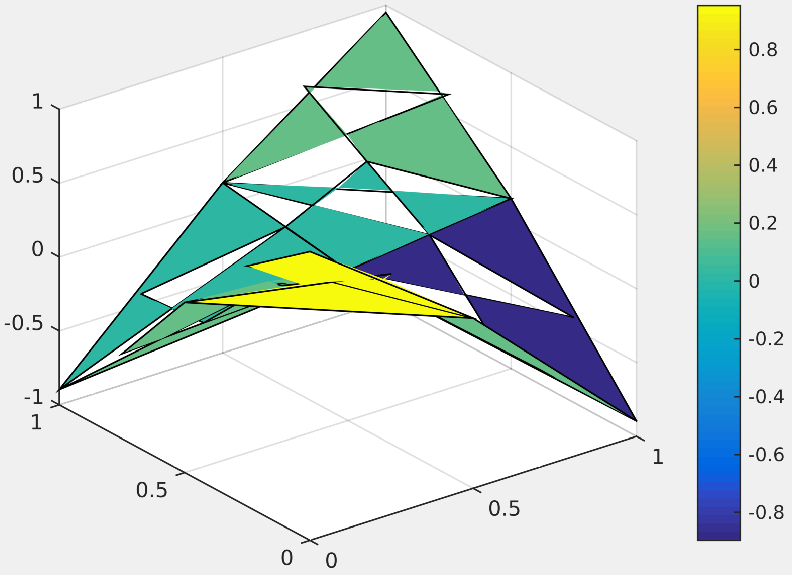
\includegraphics[scale=0.9]{appro_solution_1_P2}
\caption{$\mathbb{P}_2$ approximate solution.}
\end{figure} 

\begin{figure}[H]
\centering
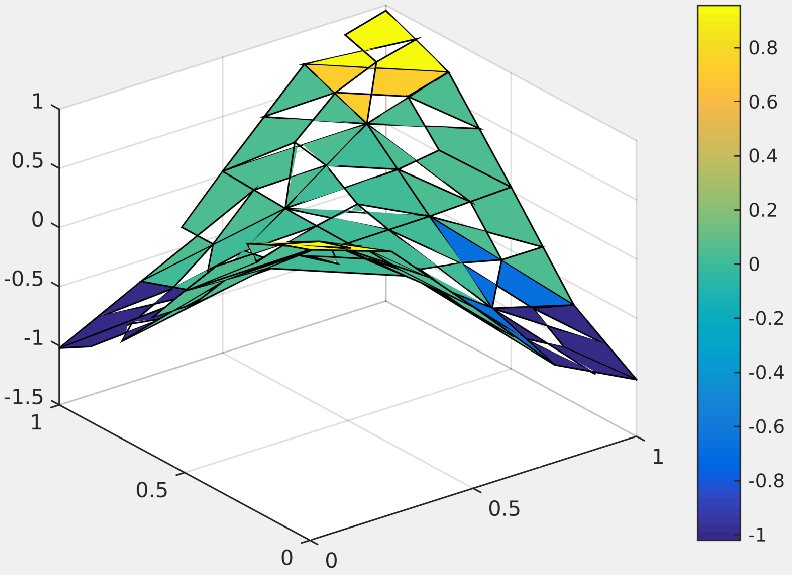
\includegraphics[scale=0.9]{appro_solution_2_P2}
\caption{$\mathbb{P}_2$ approximate solution.}
\end{figure} 

\begin{figure}[H]
\centering
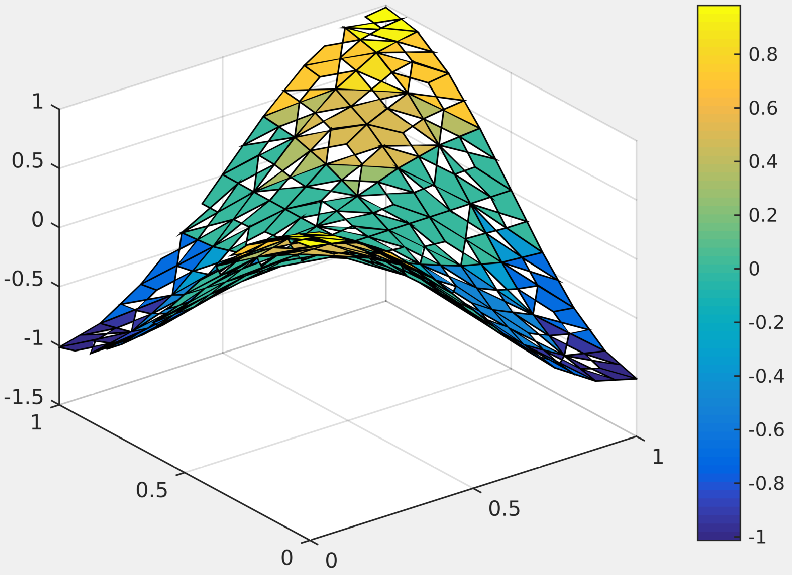
\includegraphics[scale=0.9]{appro_solution_3_P2}
\caption{$\mathbb{P}_2$ approximate solution.}
\end{figure} 

\begin{figure}[H]
\centering
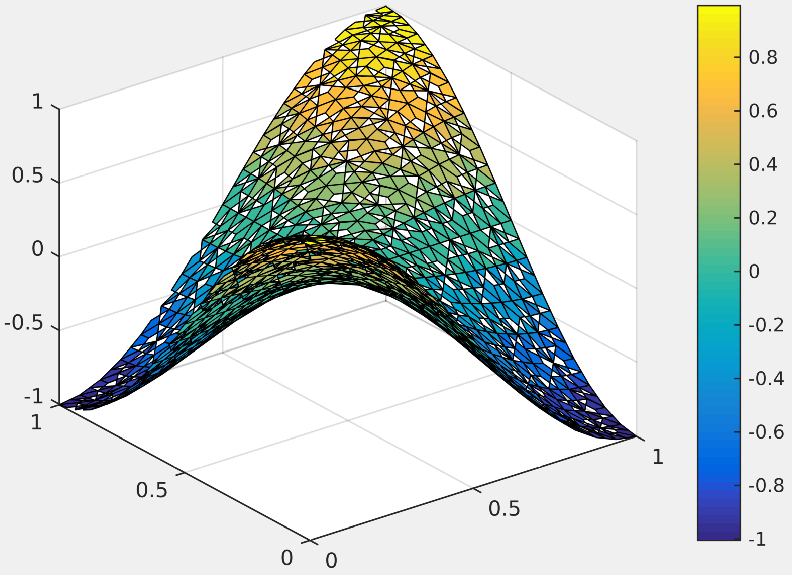
\includegraphics[scale=0.9]{appro_solution_4_P2}
\caption{$\mathbb{P}_2$ approximate solution.}
\end{figure}

\begin{figure}[H]
\centering
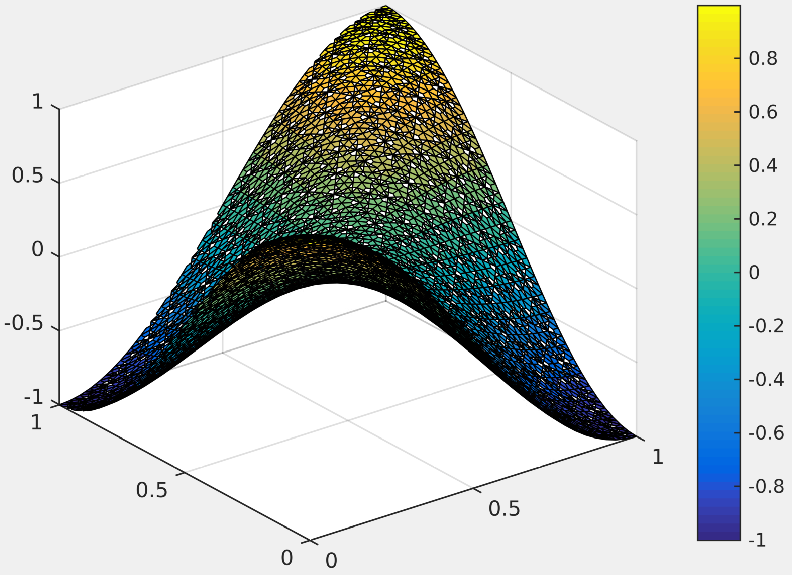
\includegraphics[scale=0.9]{appro_solution_5_P2}
\caption{$\mathbb{P}_2$ approximate solution.}
\end{figure}  

%\begin{figure}[H]
%\centering
%\includegraphics[scale=0.9]{appro_solution_6_P2}
%\caption{$\mathbb{P}_2$ approximate solution.}
%\end{figure} 
This completes our solution.
\end{proof}

\begin{prob}
Using the function defined in Problem \ref{prob2.1}, write a script which calculates the numerical solution for different values of $h$ and plot the curves of the relative errors for the euclidian and the infinity norms, with respect to $h$, in ``loglog'' scale:
\begin{itemize}
\item[(a)] for the $\mathbb{P}_1$ approximation.
\item[(b)] for the $\mathbb{P}_2$ approximation.
\end{itemize}
\end{prob}

\begin{proof}[Solution]
See Sec. \ref{sec3.5}. Running the following command lines in the main script
\begin{verbatim}
convergence_order(mesh_geo, 4, 1);
convergence_order(mesh_geo, 4, 2);
\end{verbatim}
gives us 
\begin{figure}[H]
\centering
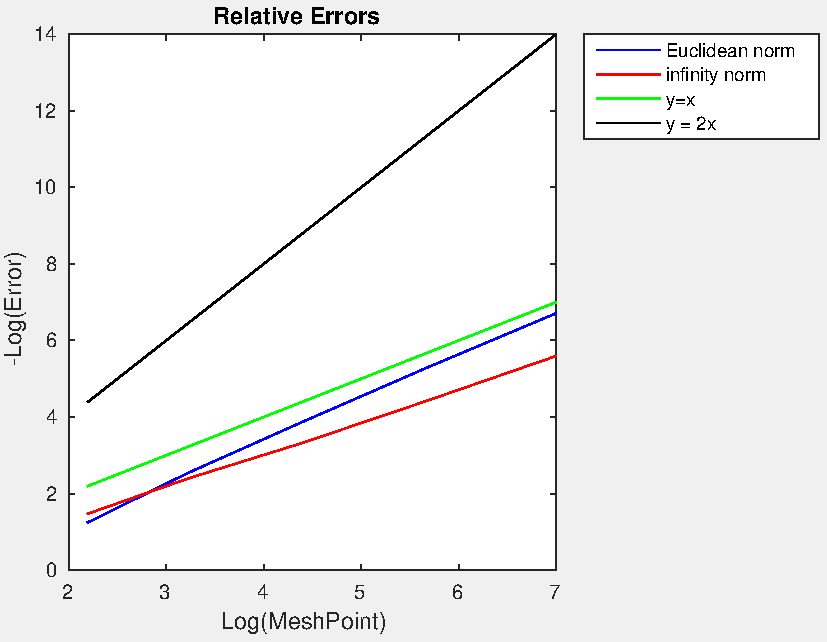
\includegraphics[scale=0.9]{convergence_order_P1}
\caption{Convergence order of the $\mathbb{P}_1$ approximation}
\end{figure}

\begin{figure}[H]
\centering
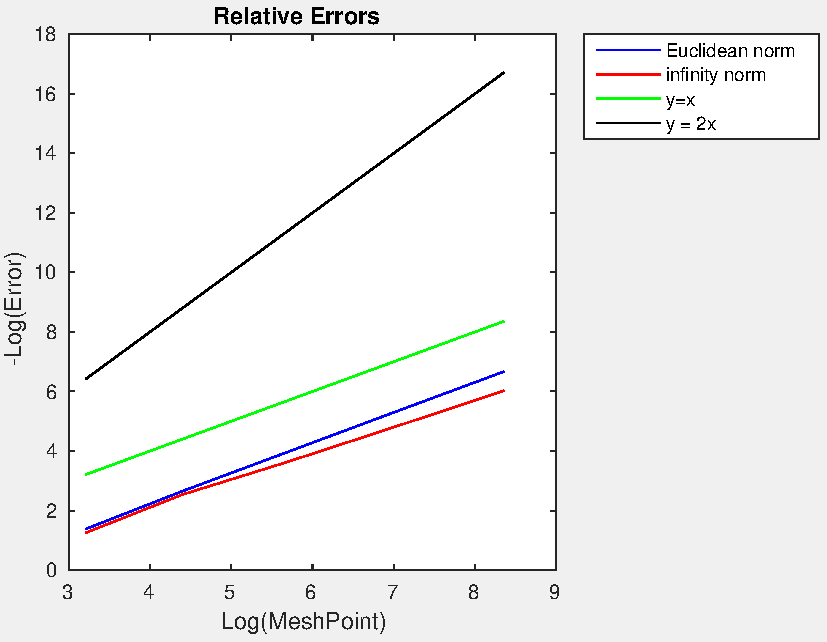
\includegraphics[scale=0.9]{convergence_order_P2}
\caption{Convergence order of the $\mathbb{P}_2$ approximation}
\end{figure}
This completes our solution.
\end{proof}


\section{Appendices: MATLAB Scripts}

\subsection{Function One}
The following \textsc{Matlab} script returns the function $f\left(x\right)=1$. 
\begin{verbatim}
function a = f_one(x)
% Evaluation of the function f(x) = 1 for all x 
% Input: 
% + x: a 1x2 or 2x1 vector
% Output:
% + a: the value 1

a = 1;
\end{verbatim}

\subsection{Exact Solution}
The following \textsc{Matlab} script returns the values of the proposed exact solution 
\begin{align}
u\left( {{x_1},{x_2}} \right) = \cos \left( {\pi {x_1}} \right)\cos \left( {\pi {x_2}} \right),\hspace{2mm}\forall \left( {{x_1},{x_2}} \right) \in {\left[ {0,1} \right]^2}.
\end{align}
\begin{verbatim}
function exact_sol = exact_solution(x,y)
% The exact solution is given by u(x) = cos(pi*x)*cos(pi*y)
% Input:
% + x: a 2x1 or 1x2 vector
% Output:
% + exact_sol: the value of the exact solution at the point x, i.e. 
% u(x,y) = cos(pi*x)*cos(pi*y)

exact_sol = cos(pi*x).*cos(pi*y);
\end{verbatim}

\subsection{Source Function}
The following \textsc{Matlab} script returns the values of the proposed source function
\begin{align}
f\left( {{x_1},{x_2}} \right) = \left( {2{\pi ^2} + 1} \right)\cos \left( {\pi {x_1}} \right)\cos \left( {\pi {x_2}} \right),\hspace{2mm}\forall \left( {{x_1},{x_2}} \right) \in {\left[ {0,1} \right]^2}.
 \end{align} 
\begin{verbatim}
function f = source_function(x)
% The source function is given by f = - Laplacian(u) + u, where u is the
% exact solution
% Input:
% + x: a 2x1 or 1x2 vector
% Output:
% + f: the value of the source function at the point x, i.e. 
% f(x1,x2) = (2*pi^2 + 1)*cos(pi*x1)*cos(pi*x2)

f = (2*pi^2 + 1)*cos(pi*x(1))*cos(pi*x(2)); 
\end{verbatim}

\subsection{Solve the Neumann Boundary Value Problem}\label{sec3.4}
The following \textsc{Matlab} script is used to solve the introduced Neumann BVP.
\begin{verbatim}
function [X, nodes] = solve_Neumann_BVP(mesh_geo, h, degree_FE)
% Solve the problem: -Laplacian(u) + u = f with the homogeneous Neumann
% boundary condition, on a domain described geometrically by mesh_geo, by 
% application of the finite-element method (isoparametric P_1 or P_2). This
% function builds the mesh (P_1 or P_2) according to the discretization
% parameter h, then assemblies the matrix of the variational approximation,
% and finally solves the linear system.
% Author: Nguyen Quan Ba Hong
% Date: 8/11/2018
% Last Update: 8/11/2018
% Inputs:
% + mesh_geo: a mesh structure defining the geometry, if degree_FE = 1,
% this mesh structure must be a P_1 mesh structure, if degree_FE = 2, it
% must be modified into a P_2 mesh structure 
% + h: discretization parameter of the mesh
% + degree_FE: degree of the finite-element interpolation
% Outputs:
% + X: a vector which contains the approximation of the exact solution at
% the nodes of the mesh
% + nodes: the coordinates of the nodes of the built mesh 

%% Refine the Mesh Given
while 1
    % Compute the Mesh Size of the Current Mesh
    [~, max_edge_size] = find_worst_triangle(mesh_geo);
    if (max_edge_size <= h) % Stopping Criteria
        break % The Current Mesh is Fine Enough
    end
    mesh_geo = refine_mesh(mesh_geo);
end

%% Choose Mesh Structure According to the Degree of the FE Interpolation
if (degree_FE == 2) % The FE Interpolation of Second Order
    mesh_geo = P1_to_P2(mesh_geo); % Modify mesh_geo into P_2 Mesh Structure
end

%% Assembling Procedures
% Compute the Mass Matrix
M =  assemble_matrix('Id', 'Id', 'f_one', mesh_geo, degree_FE, 2);
% Compute the Stiffness Matrix
R1 = assemble_matrix('D1', 'D1', 'f_one', mesh_geo, degree_FE, 1);
R2 = assemble_matrix('D2', 'D2', 'f_one', mesh_geo, degree_FE, 1);
% Assembly the Finite-Element Matrix
A = M + R1 + R2;
% Assembly the Finite-Element Right Hand Side Vector
b = assemble_vector('Id', 'source_function', mesh_geo, degree_FE, 2);

%% Resolution
X = A\b; % Solve the Linear System Ax = b
nodes = mesh_geo.coords; % the Nodes of the Current Mesh
\end{verbatim}

\subsection{Convergence Order}\label{sec3.5}
The following \textsc{Matlab} script is used to validate the convergence order of the finite-element method.
\begin{verbatim}
function [] = convergence_order(mesh_geo, times, degree_FE)
% Calculate the numerical solution for different values of the
% discretization parameter h and plot the curves of the relatives errors
% for the euclidean and the infinity norms, with respect to h, in "loglog"
% scale
% (a) for the P_1 approximation
% (b) for the P_2 approximation
% Author: Nguyen Quan Ba Hong
% Date: 8/11/2018
% Last Update: 8/11/2018
% Inputs:
% + mesh_geo: a mesh structure defining the geometry, if degree_FE = 1,
% this mesh structure must be a P_1 mesh structure, if degree_FE = 2, it
% must be modified into a P_2 mesh structure
% + times: the number of times which we refine the mesh given
% + degree_FE: degree of the finite-element interpolation
% + Output: a plot of the curves of the relative errors for the euclidean
% and the infinity norms, with respect to h, in "loglog" scale

%% Initializations
h_max = 100; % Fixed Maximal Discretization Parameter
relative_error_euclidean = zeros(times + 1,1);
relative_error_infinity = zeros(times + 1,1);
number_mesh_point = zeros(times + 1,1);

% Solve the Neumann BVP for the Initial Mesh
[X, nodes] = solve_Neumann_BVP(mesh_geo, h_max, degree_FE);
% Compute the Number of Nodes ofthe Initial Mesh
number_mesh_point(1) = size(nodes,1); 
% Compute the Exact Solution on the Initial Mesh
U_ex = zeros(size(nodes,1),1); % Initialize
for i = 1:size(nodes,1)
    U_ex(i) = exact_solution(nodes(i,1), nodes(i,2));
end
% Compute the Relative Error for the Euclidean Norm
relative_error_euclidean(1) = norm(X - U_ex,2)/norm(U_ex,2);
% Compute the Relative Error for the infinity Norm
relative_error_infinity(1) = norm(X - U_ex,Inf)/norm(U_ex,Inf);

%% Main Loop
for i = 1:times % Refine the Inputted Mesh times Times
    mesh_geo = refine_mesh(mesh_geo); % Refine the Current Mesh
    [X, nodes] = solve_Neumann_BVP(mesh_geo, h_max, degree_FE);
    % Compute the Number of Nodes of the Current Mesh
    number_mesh_point(i+1) = size(nodes,1);
    % Compute the Exact Solution on the Initial Mesh
    U_ex = zeros(size(nodes,1),1); % Initialize
    for j = 1:size(nodes,1)
        U_ex(j) = exact_solution(nodes(j,1), nodes(j,2));
    end
    % Compute the Relative Error for the Euclidean Norm
    relative_error_euclidean(i+1) = norm(X - U_ex,2)/norm(U_ex,2);
    % Compute the Relative Error for the infinity Norm
    relative_error_infinity(i+1) = norm(X - U_ex,Inf)/norm(U_ex,Inf);
end

%% Plot the Relative Errors in the "loglog" Scale
figure
plot(log(number_mesh_point), -log(relative_error_euclidean), 'blue',...
     log(number_mesh_point), -log(relative_error_infinity), 'red',...
     log(number_mesh_point), 2*log(number_mesh_point), 'green');
xlabel('Log(MeshPoint)');ylabel('-Log(Error)');
title('Relative Errors');
legend('Euclidean norm','infinity norm', 'y = 2x','Location','NorthEastOutside');  
\end{verbatim}





%\section*{Appendix A. Supplementary notes}



%\section*{Acknowledgment}

\newpage
\begin{thebibliography}{999}
\bibitem {1} \url{https://perso.univ-rennes1.fr/eric.darrigrand-lacarrieu/Teaching/M2RFEorganisation.html}
\end{thebibliography}
%\bibliographystyle{siam}
%\bibliography{MYBIB}
%\Addresses
\end{document}
